\DocumentMetadata{
  pdfversion=2.0,
  lang=es-MX,
  pdfstandard=ua-2
}

\documentclass{sener2025}

\addbibresource{referencias.bib}

% --- Metadatos PDF/UA (Accesibilidad Universal) ---
\hypersetup{
  pdftitle={Balance Nacional de energía 2024},
  pdfauthor={Equipo de Planeación (demo)},
  pdfsubject={Ejemplos de secciones, etiquetas y bloques (para pruebas del generador)},
  pdfkeywords={SENER, Energía, México},
  pdfcreationdate={D:20251216084914},
  pdfversion={1}
}

% --- Metadatos del Documento ---
\title{Balance Nacional de energía 2024}
\subtitle{Ejemplos de secciones, etiquetas y bloques (para pruebas del generador)}
\author{Equipo de Planeación (demo)}
\date{14 de diciembre de 2025}
\institucion{Secretaría de Energía (SENER)}
\unidad{Unidad de Planeación y Transición Energética}
\setDocumentoCorto{BNE-2025}
\palabrasclave{}
\version{1}

\begin{document}

\portadafondo[img/portada.png]

\tableofcontents
\newpage

\listafiguras
\newpage

\listatablas
\newpage

\clearpage
\begin{center}
{\Large\patriafont\bfseries\color{gobmxGuinda}Agradecimientos}\\[1cm]
\end{center}

Agaredecemos a:
1.-JAvi;
2.-Diego;
3.-Rodrigo;

\clearpage
\begin{center}
{\Large\patriafont\bfseries\color{gobmxGuinda}Presentación}\\[1cm]
\end{center}

La Seguridad Energética es un objetivo estratégico del Plan Nacional de Desarrollo 2025-2030, pero debe hacerse con una visión de sustentabilidad ambiental; para ello es fundamental consolidar la rectoría del Estado en el sector energético mediante el fortalecimiento de PEMEX y de la CFE. Esto permitirá eliminar la dependencia del exterior, asegurar precios accesibles para la población y avanzar hacia la autosuficiencia energética. En la matriz energética del país se impulsarán fuentes de energía renovables y se acelerará la transición energética con el objetivo de reducir las emisiones contaminantes, cumplir con las metas nacionales de energías limpias y honrar los compromisos internacionales en la lucha contra el cambio climático.

 Además de garantizar un suministro energético seguro, eficiente y asequible para toda la población, la justicia energética debe convertirse en un pilar del desarrollo nacional. Esto implica ampliar la cobertura y el acceso a la energía, especialmente en comunidades marginadas, asegurando que todas las regiones del país cuenten con fuentes de energía limpias y sostenibles.

 En México se ha tomado la decisión de trabajar con una visión de preservar la seguridad y autosuficiencia energética, encaminarse a una transición energética justa y sustentable, así como de brindar certeza jurídica a las actividades que se realizan en el sector. Por estas razones, se han hecho cambios al marco jurídico del sector energético partiendo de las modificaciones a la Constitución Política de los Estados Unidos Mexicanos y a diversos ordenamientos jurídicos que de ella emanan. En este sentido, la SENER tiene el mandato legal de ser el órgano rector de la política y planeación energética nacional, bajo criterios de soberanía y seguridad energética, autosuficiencia, restitución y aumento de reservas, diversificación de fuentes de combustibles, mejoramiento de la productividad, la reducción progresiva de impactos ambientales en la producción y consumo de energía, y la satisfacción de las necesidades energéticas básicas mediante cobertura universal a toda la población a precios accesibles.

 Secretaría de Energía

\clearpage
\begin{center}
{\Large\patriafont\bfseries\color{gobmxGuinda}Resumen Ejecutivo}\\[1cm]
\end{center}

Este documento es un banco de pruebas. Incluye ejemplos de:
• Listas
• Etiquetas inline (nota, cita, math)
• Bloques (recuadro, ejemplo, info, alerta)
• Anexos
• Tablas y figuras

Objetivo: detectar errores de escape y de parsing antes de publicar.

\clearpage
\begin{center}
{\Large\patriafont\bfseries\color{gobmxGuinda}Datos Clave}\\[1cm]
\end{center}

\begin{itemize}
  \item Dato 1
  \item Dato 2
  \item Dato 3
  \item Dato 4
\end{itemize}

\portadaseccion{1}{Introducción}{x......}

\section{Introducción}

El sector energético es un área estratégica para el funcionamiento de la economía y el bienestar de la sociedad mexicana, ya que proporciona energía para el desarrollo nacional a través de los sectores agropecuario, industrial, residencial, comercial, transporte, de servicios públicos, entre otros. También, suministra insumos para fines no energéticos en la industria petroquímica, como es la producción de fertilizantes, medicamentos y plásticos ampliamente utilizados en un sin número de artículos de uso cotidiano.

Con el propósito de comprender y analizar la dinámica energética del país, así como de generar la base para la planeación vinculante, la Secretaría de Energía (SENER) elabora anualmente el Balance Nacional de Energía (BNE). Actualmente, este instrumento se desarrolla en el marco de la Reforma Energética de 2025, lo que le otorga un papel fundamental en la definición de políticas y estrategias para el sector.

En este documento se analiza el desempeño y la evolución del sector energético de México durante el periodo 2010-2024, con especial énfasis en el año 2024, a fin de comprender su comportamiento histórico. Por lo tanto, este análisis describe las fuentes de energía, su transformación y el consumo final de energía durante 2024. A partir de ello, el BNE busca evaluar el sector energético de México y poner a disposición del público información sobre toda la cadena de valor, que abarca la producción y el consumo de energía primaria y secundaria.
Además, esta información es esencial para desarrollar los instrumentos de planeación del sector energético, evaluar su desempeño, así como para el diseño de políticas públicas y la toma de decisiones estratégicas alineados al Plan Nacional de Desarrollo (PND) 2025-2030 y al Programa Sectorial de Energía (PROSENER) 2025-2030.

El BNE se basa únicamente en un análisis energético, por lo que excluye aspectos económicos como el Producto Interno Bruto (PIB), los precios y las tarifas de la energía o la inflación. Esto se debe a que el documento ofrece un panorama general sobre el sector energético a partir de las bases energéticas objetivas con las que cuenta el país, con lo que se ofrece, no solo una visión del presente, sino una proyección del futuro energético de México.

\begin{figure}[H]
  {\centering
  % Texto alternativo para accesibilidad
  \pdftooltip{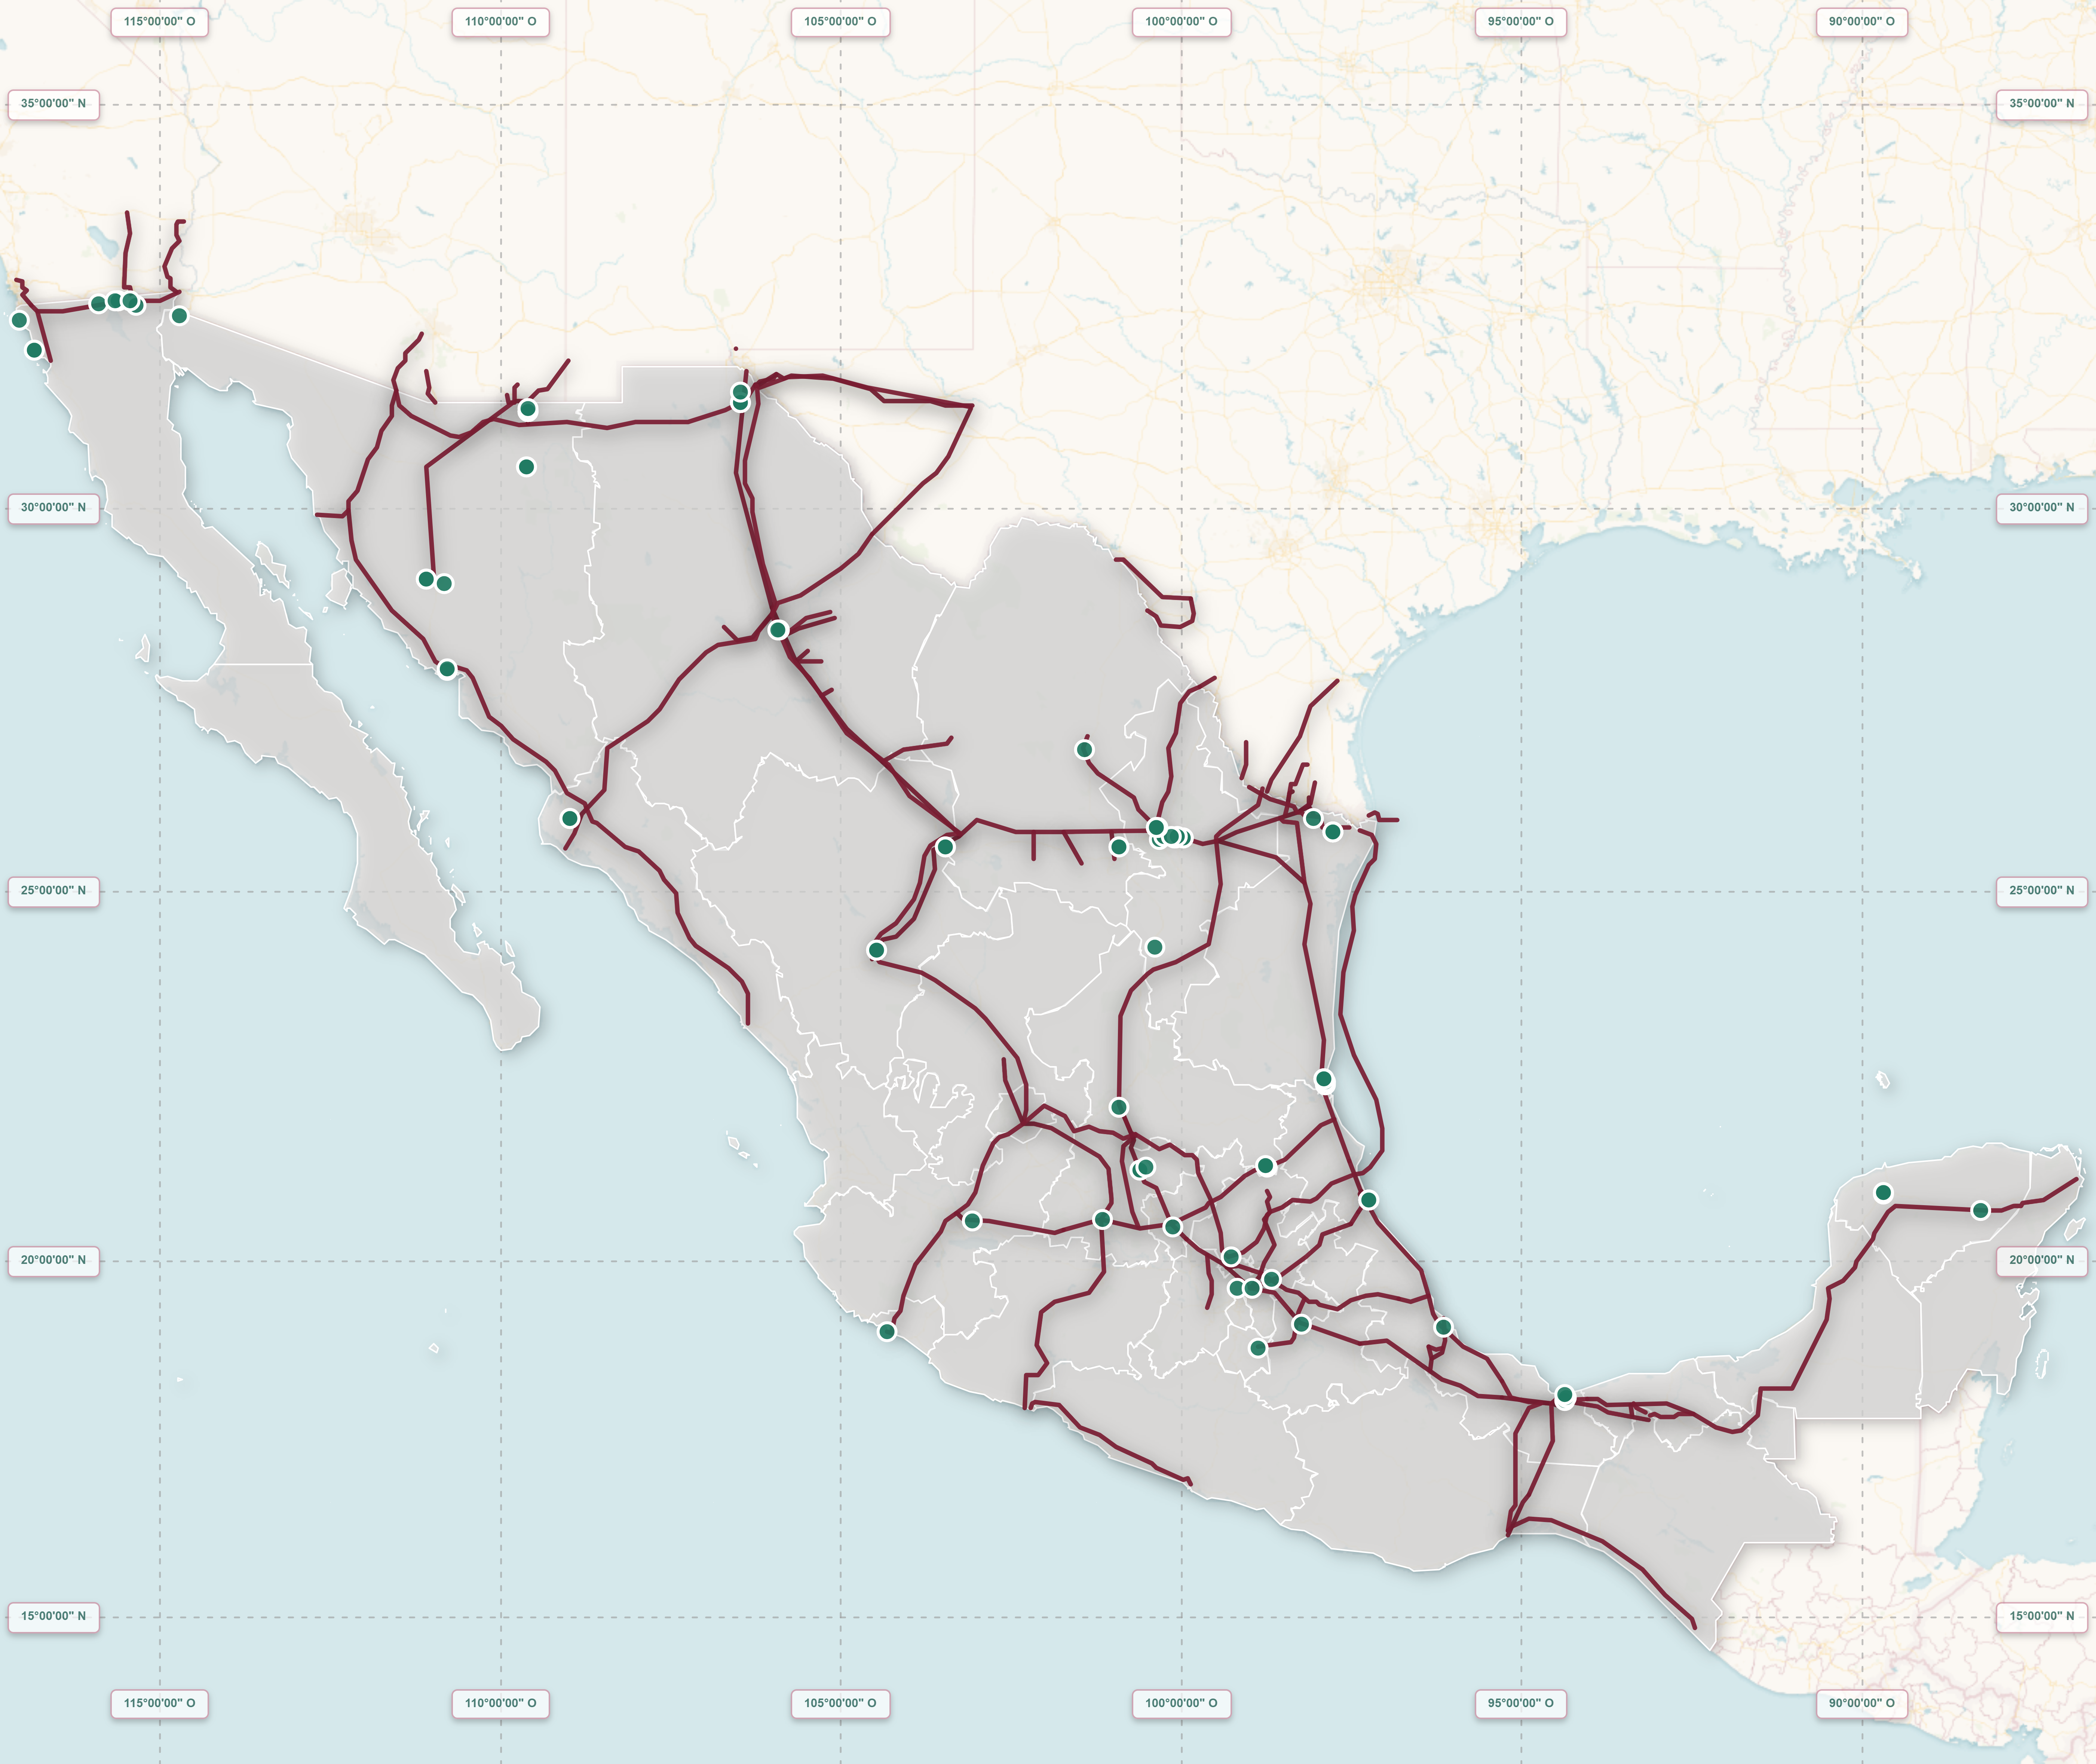
\includegraphics[width=0.8\textwidth]{img/graficos/figura_2_12.png}}{Gráfica circular (pie chart) que muestra la distribución porcentual del consumo energético en México por sector económico durante 2024. Sector industrial: 45\% (color guinda), sector transporte: 30\% (verde), sector residencial: 15\% (dorado), otros sectores: 10\% (gris). Total: 100\% equivalente a 4,250 petajoules.}
  \par}
  \raggedright
  \caption{Distribución del consumo final de energía por sector, 2024}
  \label{fig:distribucion_del_consumo_final}
\end{figure}
\vspace{-4pt}
\fuente{Elaboración propia con datos de CENACE y CRE

{\fontsize{9pt}{11pt}\selectfont
\begin{itemize}
  \item[\hypertarget{nota1}{1/}] Incluye generación distribuida
  \item[\hypertarget{nota2}{2/}] Datos preliminares para 2025
\end{itemize}
}}

\begin{tabladoradoCorto}
  \caption{Tabla Diego}
  \label{tab:tabla_diego}
  \begin{tabular}{H{3cm}G{2cm}G{2cm}}
    \toprule
    \rowcolor{gobmxDorado} \encabezadodorado{\textbf{Concepto}} & \encabezadodorado{Val1} & \encabezadodorado{tres} \\
    \midrule
    1 & 2 & 3 \\
    \bottomrule
  \end{tabular}
\end{tabladoradoCorto}
\vspace{-4pt}
\fuente{Test}



\subsection{Fundamento jurídico del Balance Nacional de Energía}

El BNE 2024 se elabora en el marco de la Reforma Constitucional sobre áreas y empresas estratégicas y en materia de simplificación orgánica aprobadas en octubre y diciembre de 2024 , la cual constituye un hito histórico para dar entrada a la nueva política energética del Estado mexicano. La reforma, que se articula en torno a la modificación de los artículos 25, 27 y 28 de la Constitución Política de los Estados Unidos Mexicanos (CPEUM), se consolidó con la armonización de la legislación secundaria, que comprendió la expedición de ocho nuevas leyes y la modificación a tres leyes asociadas que, en su conjunto, fortalecen la rectoría del Estado en el sector energético.

Este nuevo orden normativo tiene como ejes fundamentales garantizar la seguridad y autosuficiencia energéticas, fortalecer la soberanía nacional, consolidar a la Comisión Federal de Electricidad (CFE) y Petróleos Mexicanos (PEMEX) como Empresas Públicas del Estado al servicio del pueblo, fortalecer a los demás organismos públicos del sector y robustecer las capacidades del Estado para ejercer una planeación vinculante, eficaz y estratégica. Asimismo, incorpora el principio de Justicia Energética que coloca en el centro de la acción gubernamental el acceso universal a energía asequible, segura y limpia para la atención de necesidades básicas, así como el combate frontal al comercio ilícito de combustibles y la transición energética sustentable, con una visión de largo plazo que armoniza el desarrollo económico con la protección del medio ambiente.

El papel rector y estratégico del Estado en el sector energético nacional, así como el aprovechamiento de los recursos naturales contenidos en el subsuelo (propiedad inalienable e imprescriptible de la Nación), se ejerce a través de las empresas públicas, sin que ello implique el establecimiento de monopolios, conforme lo disponen los artículos 27 y 28 constitucionales.

De acuerdo con el artículo 28 constitucional y con lo dispuesto en el artículo 20 de la Ley del Sector Eléctrico (LSE), en los artículos 4, 6 y 7 de la Ley del Sector Hidrocarburos (LSH) y el artículo 2 de la Ley de Planeación y Transición Energética (LPTE), ambas leyes reglamentarias de los artículos 25, 27 y 28 de la CPEUM, la SENER es la encargada de conducir la política energética nacional. Para ello, la SENER requiere elaborar



\section*{Glosario}
\phantomsection
\addcontentsline{toc}{section}{Glosario}

\entradaGlosario{Eficiencia energética}{Relación entre la energía útil obtenida y la energía consumida para lograr un servicio.}
\entradaGlosario{Energías renovables variables}{Tecnologías cuya generación depende del recurso (viento, solar) y fluctúa en el tiempo.}
\entradaGlosario{Flexibilidad del sistema}{Capacidad del sistema eléctrico para responder a variaciones de oferta/demanda, especialmente con renovables variables.}

\printbibliography

\section*{Siglas y Acrónimos}
\phantomsection
\addcontentsline{toc}{section}{Siglas y Acrónimos}

\entradaSigla{CENACE}{Centro Nacional de Control de Energía}
\entradaSigla{CRE}{Comisión Reguladora de Energía}
\entradaSigla{SENER}{Secretaría de Energía}


\end{document}
